\documentclass{article}
\usepackage{tikz}

\begin{document}
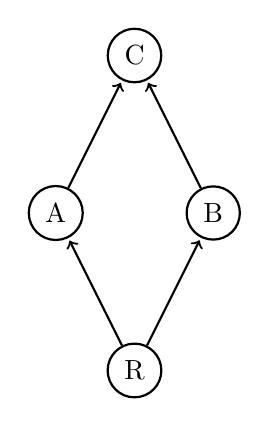
\begin{tikzpicture}[->,shorten >=1pt,auto,node distance=2.5cm, thick]

\node[circle, draw, fill=white] (R) at (0,0) {R};
\node[circle, draw, fill=white] (A) at (-1,2) {A};
\node[circle, draw, fill=white] (B) at (1,2) {B};
\node[circle, draw, fill=white] (C) at (0,4) {C};

\path (R) edge (A)
          edge (B)
      (A) edge (C)
      (B) edge (C);
      
\end{tikzpicture}


\vspace{20pt}

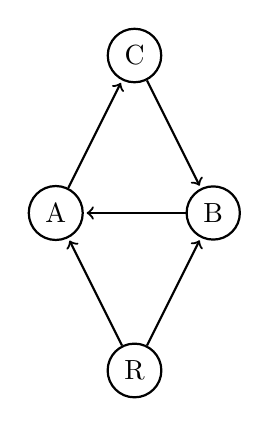
\begin{tikzpicture}[->,shorten >=1pt,auto,node distance=2.5cm, thick]

\node[circle, draw, fill=white] (R) at (0,0) {R};
\node[circle, draw, fill=white] (A) at (-1,2) {A};
\node[circle, draw, fill=white] (B) at (1,2) {B};
\node[circle, draw, fill=white] (C) at (0,4) {C};

\path (R) edge (A)
          edge (B)
      (A) edge (C)
      (C) edge (B)
      (B) edge (A);
      
\end{tikzpicture}


\end{document}
